\begin{figure}[htpb]
	\centering\capstart{}
	\subfloat[\(\mu_{1}=1.000000\)]
	{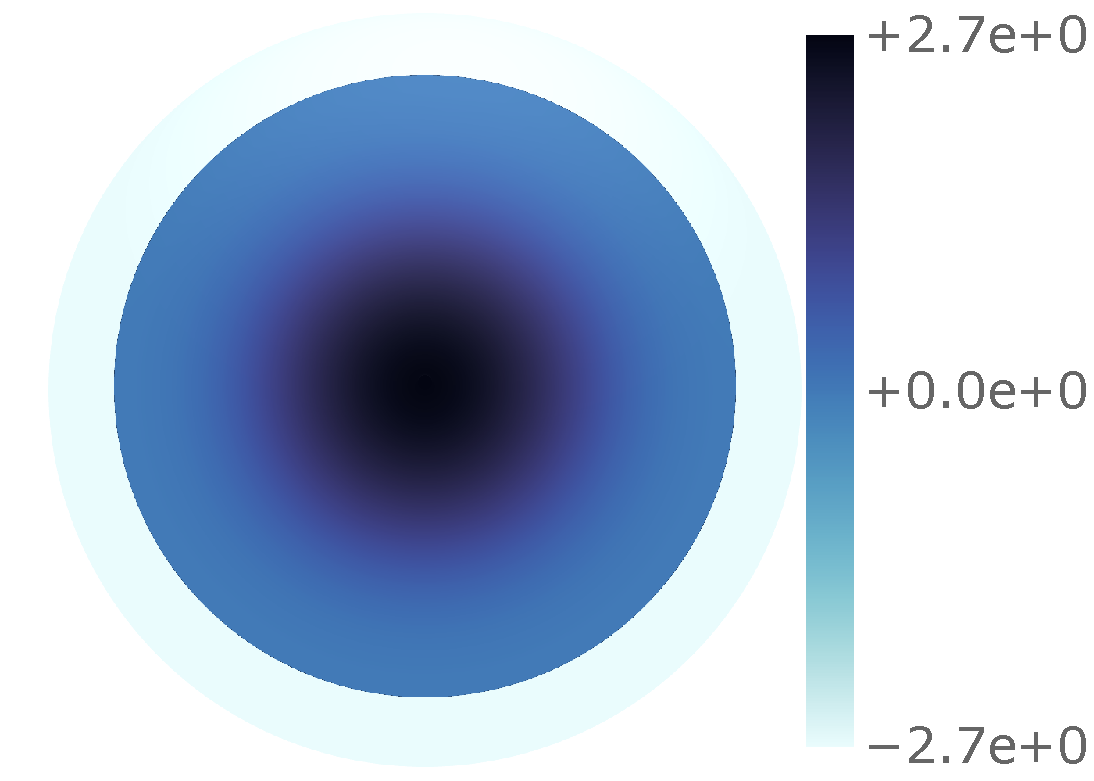
\includegraphics[trim={23 7 3 6},clip,width=.25\textwidth]{slepian_polar40_m0_rank0_lam1-000000e00_L16_res128_real.pdf}} % chktex 8
	\hfill
	\subfloat[\(\mu_{2}=0.999998\)]
	{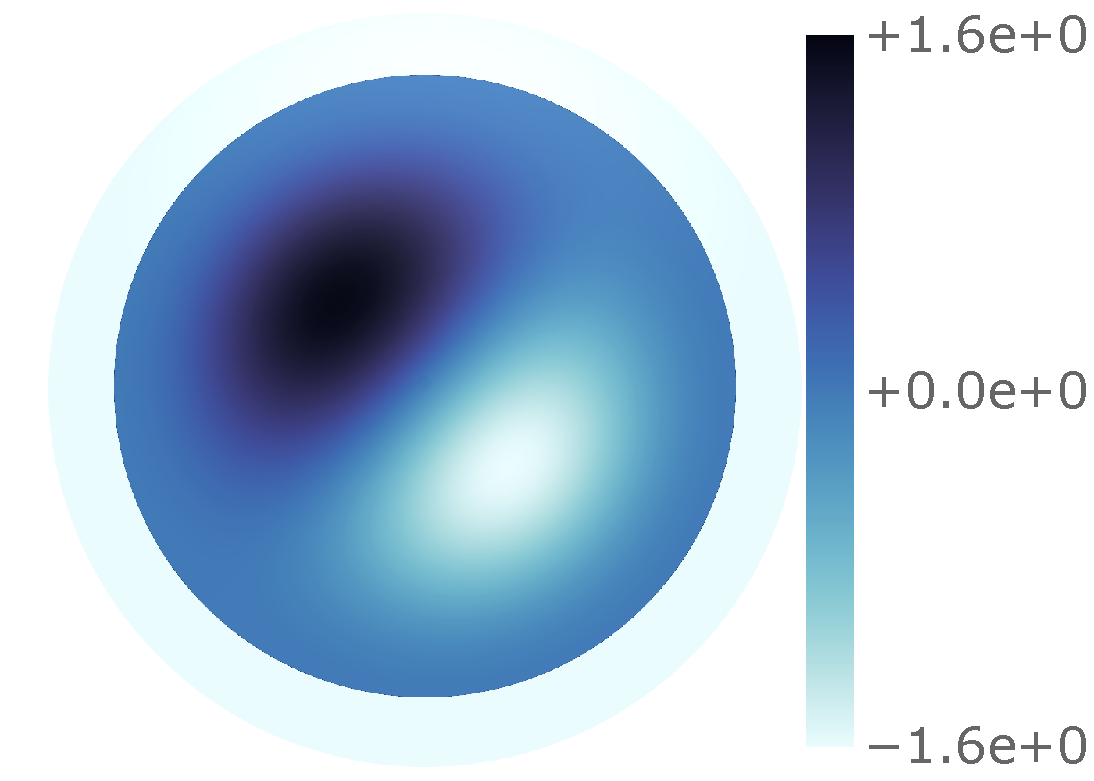
\includegraphics[trim={23 7 3 6},clip,width=.25\textwidth]{slepian_polar40_m-1_rank1_lam9-999984e-01_L16_res128_real.pdf}} % chktex 8
	\hfill
	\subfloat[\(\mu_{3}=0.999998\)]
	{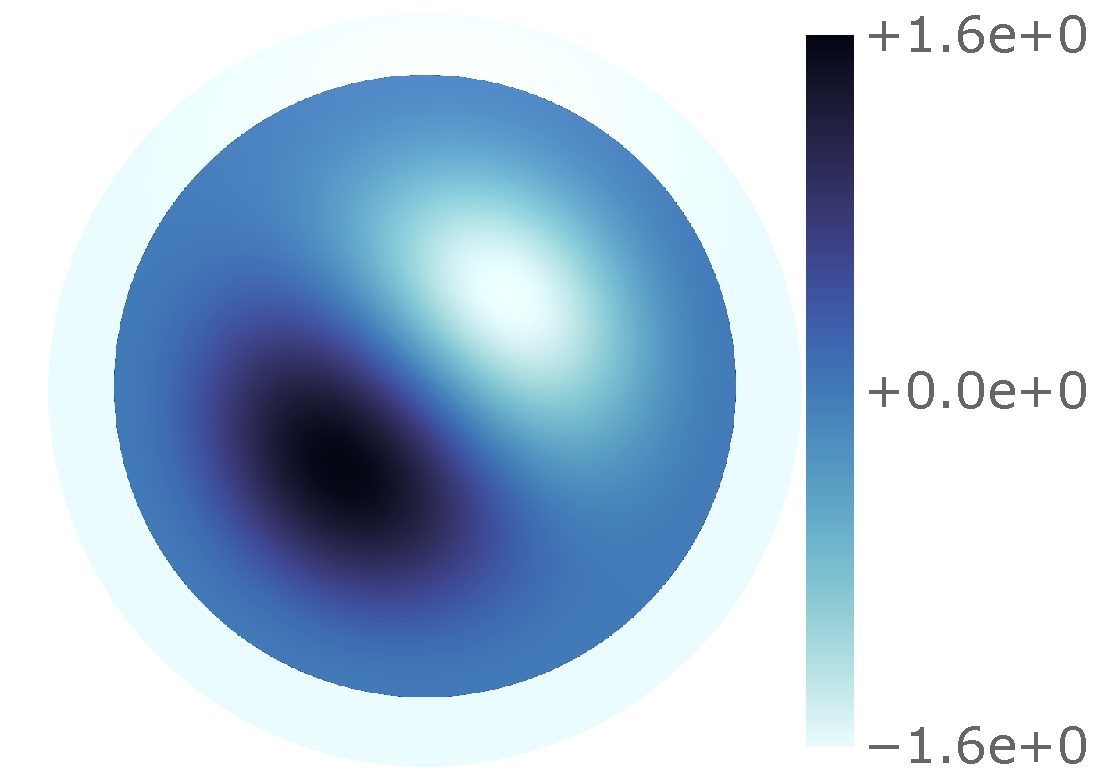
\includegraphics[trim={23 7 3 6},clip,width=.25\textwidth]{slepian_polar40_m1_rank2_lam9-999984e-01_L16_res128_real.pdf}} % chktex 8
	\hfill
	\subfloat[\(\mu_{4}=0.999966\)]
	{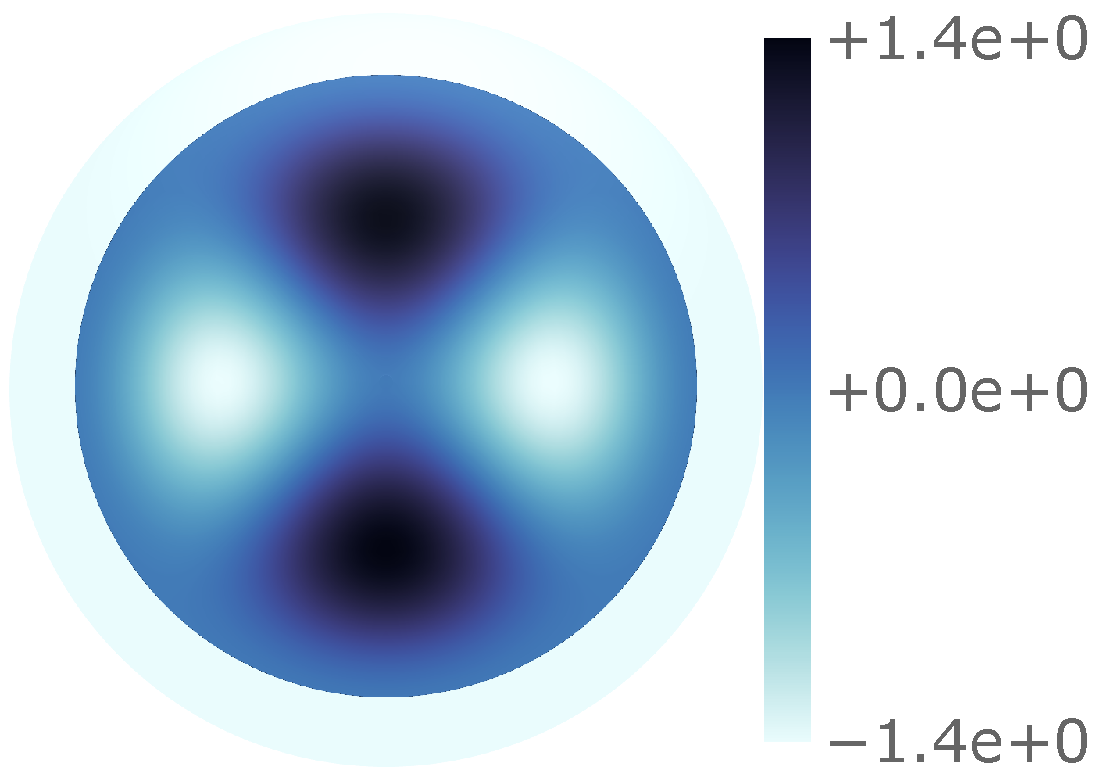
\includegraphics[trim={23 7 3 6},clip,width=.25\textwidth]{slepian_polar40_m-2_rank3_lam9-999664e-01_L16_res128_real.pdf}} % chktex 8
	\newline
	\subfloat[\(\mu_{5}=0.999966\)]
	{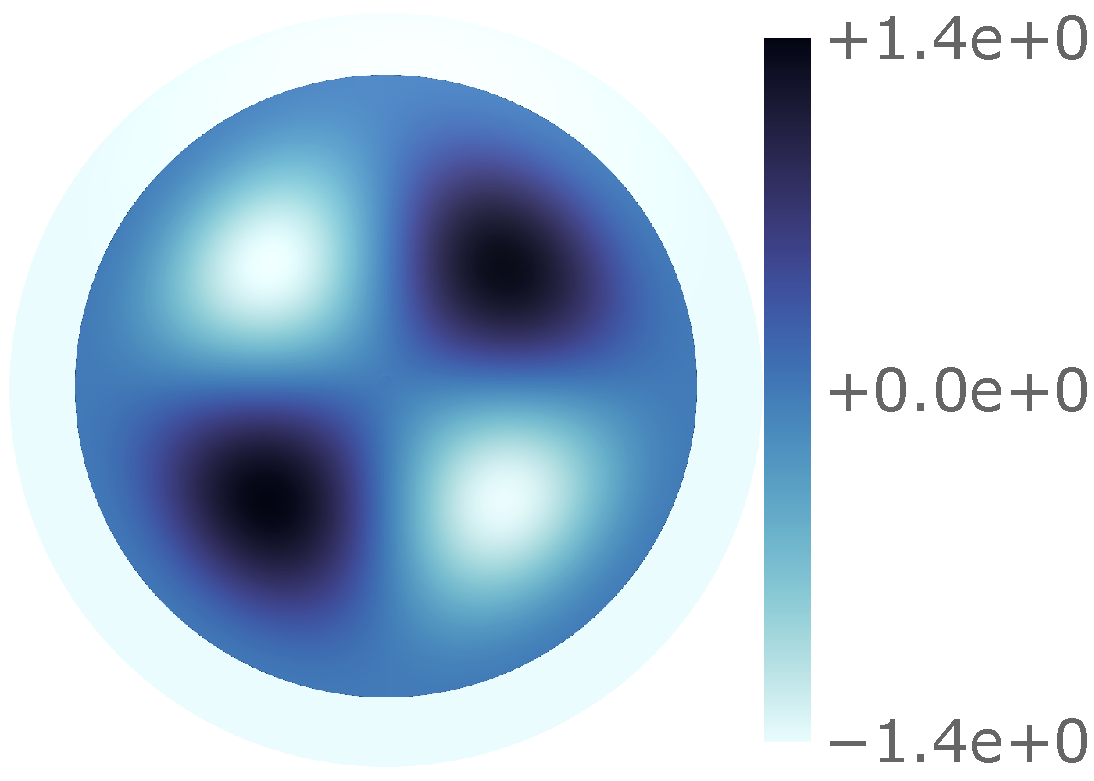
\includegraphics[trim={23 7 3 6},clip,width=.25\textwidth]{slepian_polar40_m2_rank4_lam9-999664e-01_L16_res128_real.pdf}} % chktex 8
	\hfill
	\subfloat[\(\mu_{6}=0.999939\)]
	{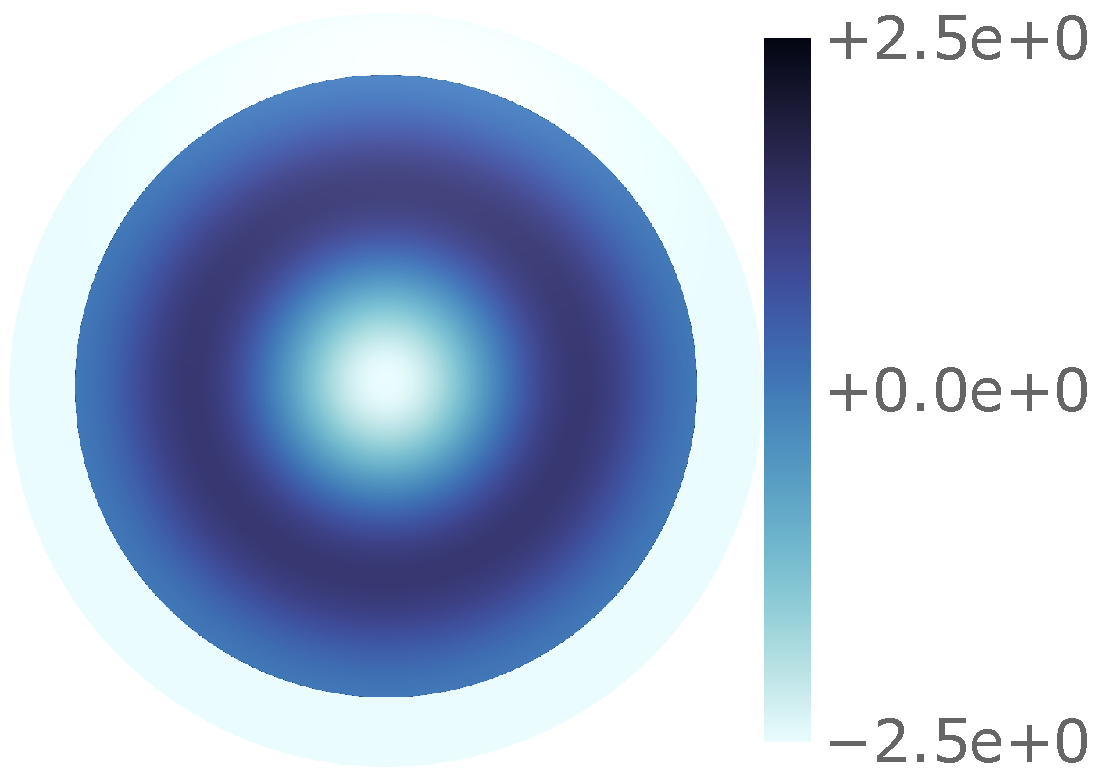
\includegraphics[trim={23 7 3 6},clip,width=.25\textwidth]{slepian_polar40_m0_rank5_lam9-999392e-01_L16_res128_real.pdf}} % chktex 8
	\hfill
	\subfloat[\(\mu_{7}=0.999553\)]
	{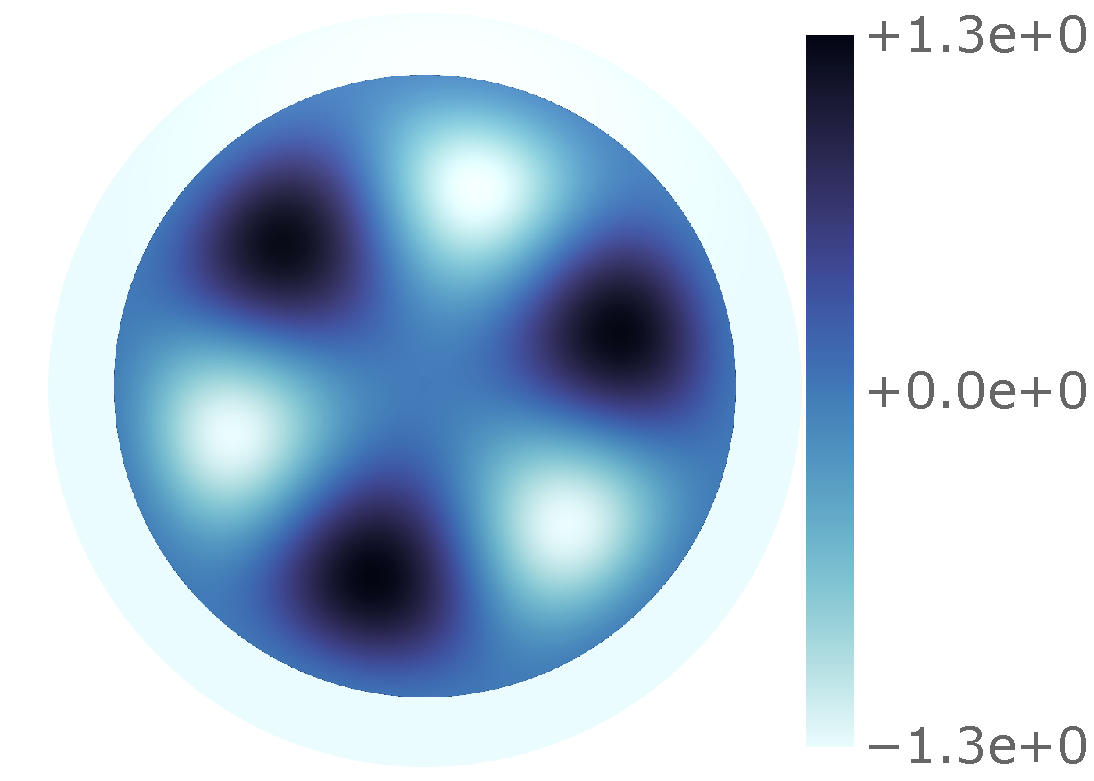
\includegraphics[trim={23 7 3 6},clip,width=.25\textwidth]{slepian_polar40_m-3_rank6_lam9-995528e-01_L16_res128_real.pdf}} % chktex 8
	\hfill
	\subfloat[\(\mu_{8}=0.999553\)]
	{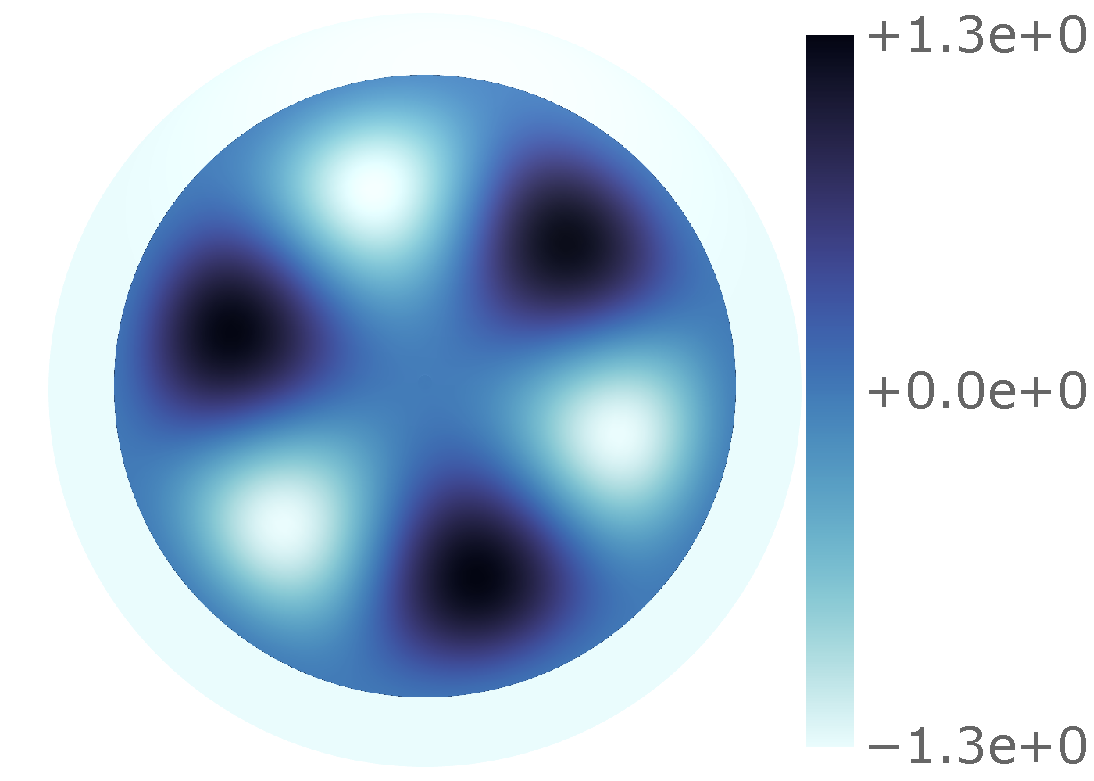
\includegraphics[trim={23 7 3 6},clip,width=.25\textwidth]{slepian_polar40_m3_rank7_lam9-995528e-01_L16_res128_real.pdf}} % chktex 8
	\newline
	\subfloat[\(\mu_{9}=0.998918\)]
	{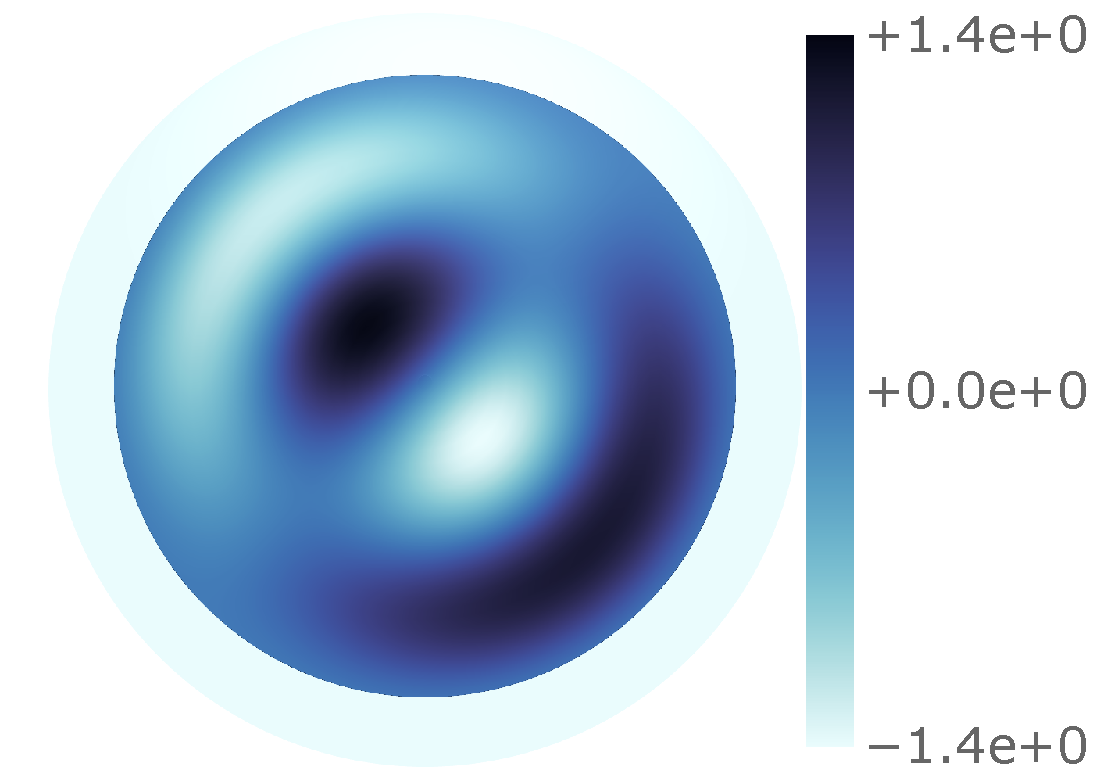
\includegraphics[trim={23 7 3 6},clip,width=.25\textwidth]{slepian_polar40_m-1_rank8_lam9-989180e-01_L16_res128_real.pdf}} % chktex 8
	\hfill
	\subfloat[\(\mu_{10}=0.998918\)]
	{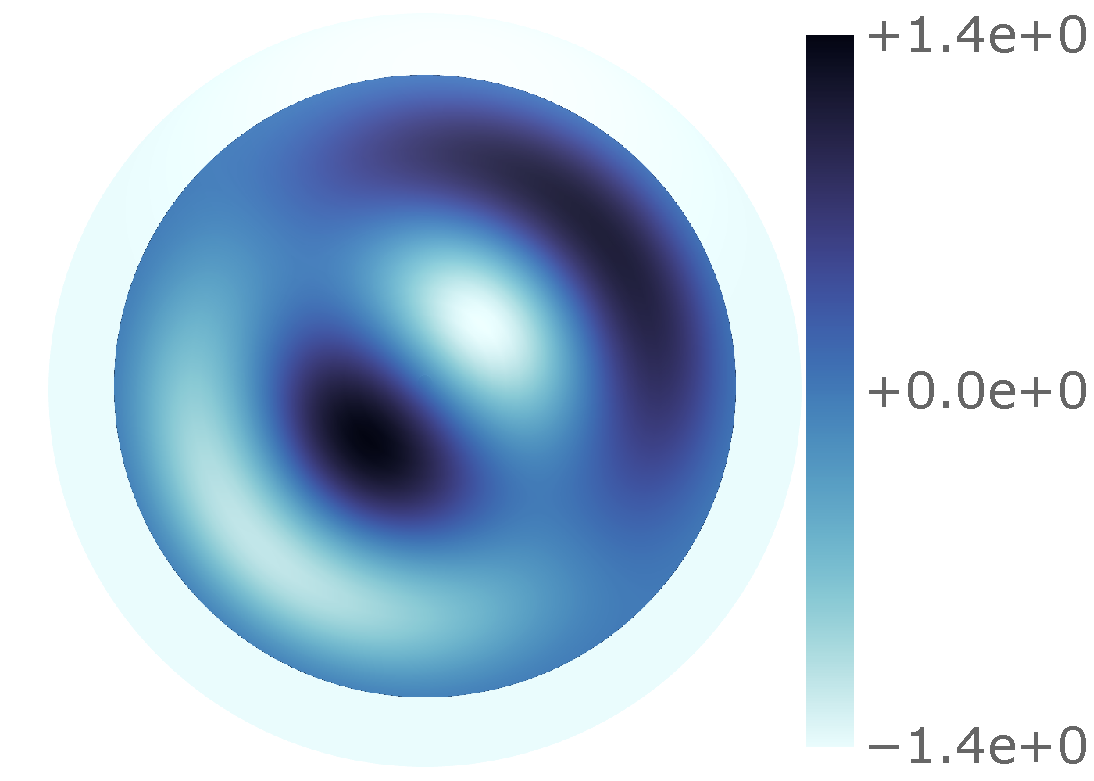
\includegraphics[trim={23 7 3 6},clip,width=.25\textwidth]{slepian_polar40_m1_rank9_lam9-989180e-01_L16_res128_real.pdf}} % chktex 8
	\hfill
	\subfloat[\(\mu_{11}=0.995897\)]
	{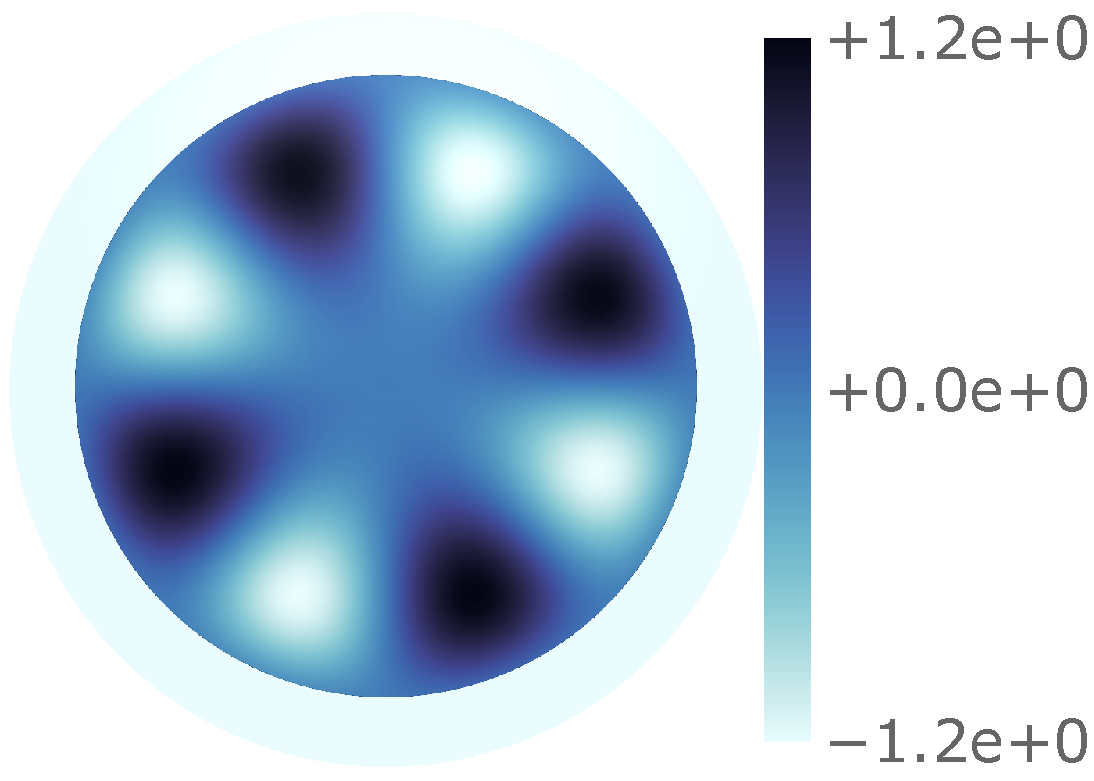
\includegraphics[trim={23 7 3 6},clip,width=.25\textwidth]{slepian_polar40_m-4_rank10_lam9-958971e-01_L16_res128_real.pdf}} % chktex 8
	\hfill
	\subfloat[\(\mu_{12}=0.995897\)]
	{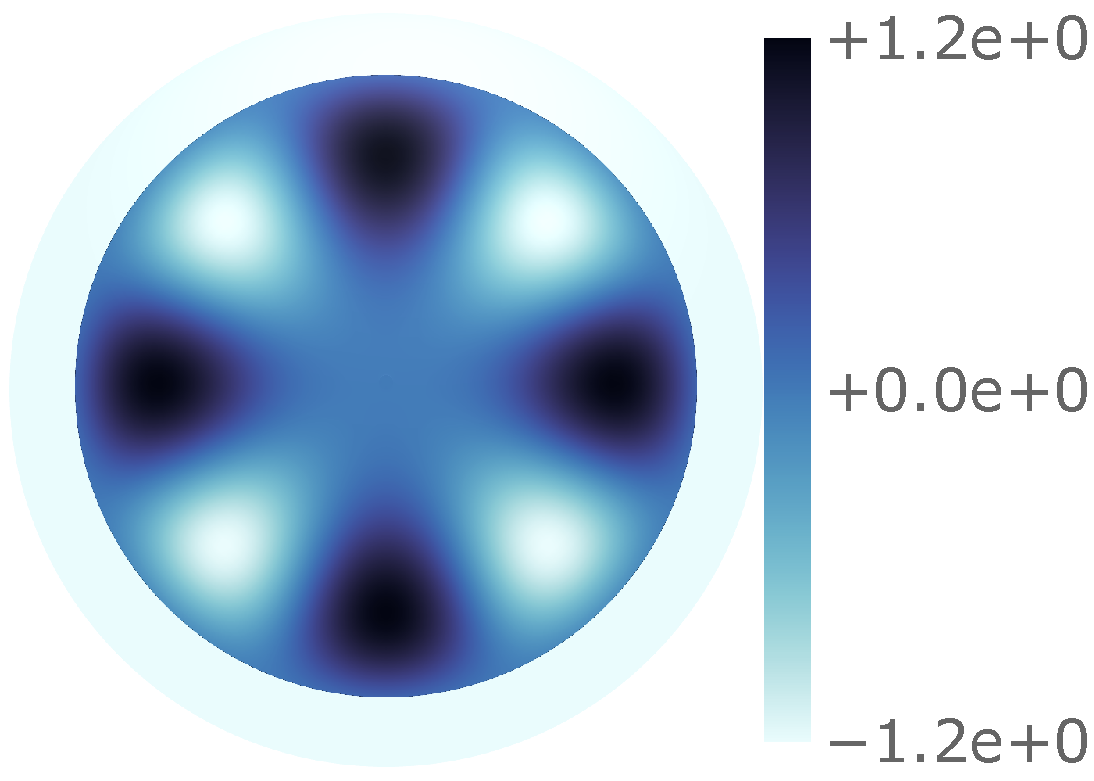
\includegraphics[trim={23 7 3 6},clip,width=.25\textwidth]{slepian_polar40_m4_rank11_lam9-958971e-01_L16_res128_real.pdf}} % chktex 8
	\newline
	\subfloat[\(\mu_{13}=0.988469\)]
	{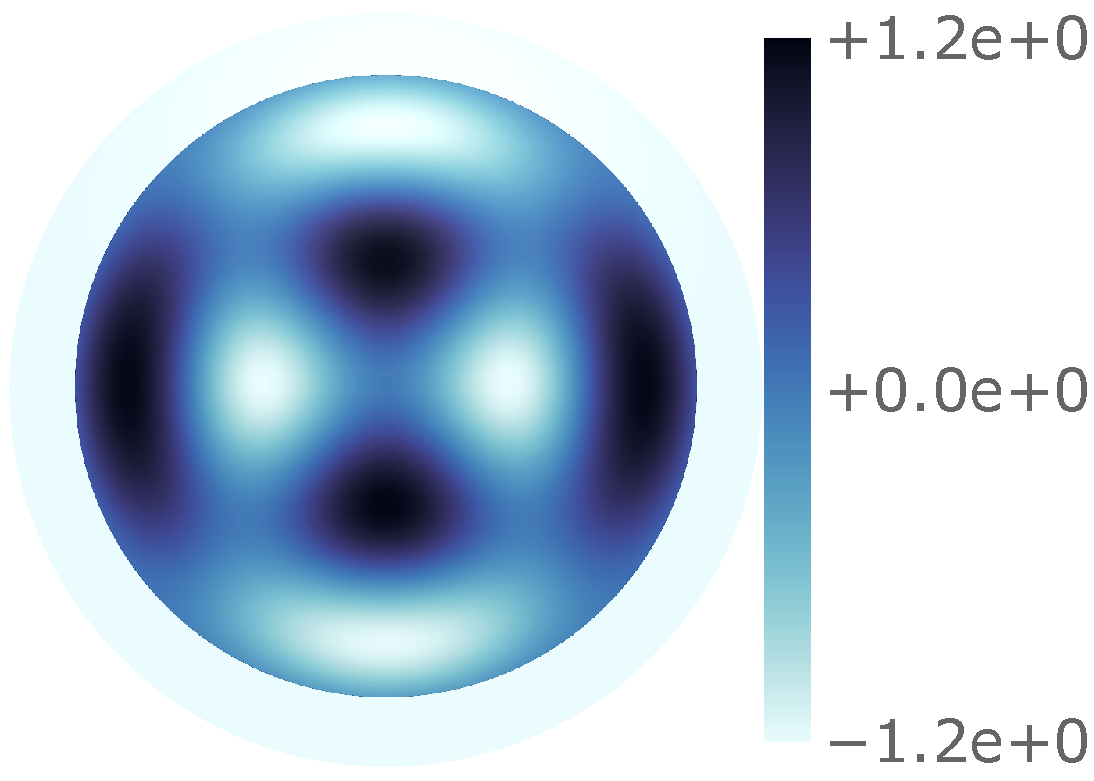
\includegraphics[trim={23 7 3 6},clip,width=.25\textwidth]{slepian_polar40_m-2_rank13_lam9-884688e-01_L16_res128_real.pdf}} % chktex 8
	\hfill
	\subfloat[\(\mu_{14}=0.988469\)]
	{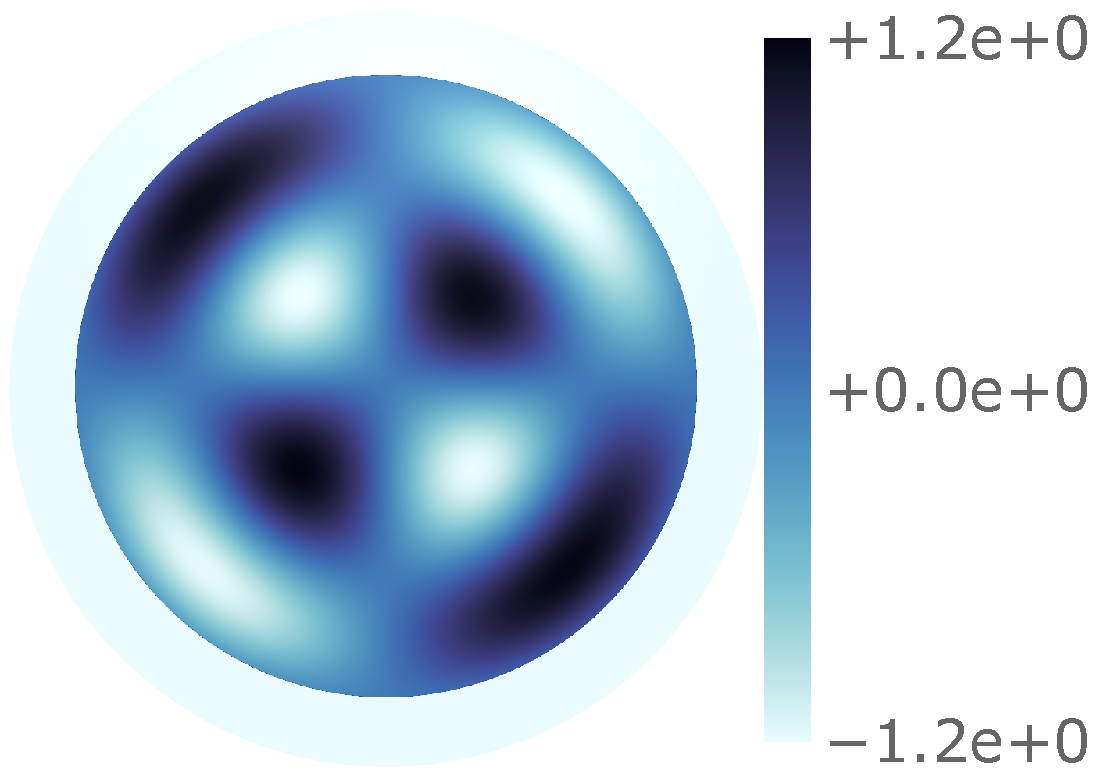
\includegraphics[trim={23 7 3 6},clip,width=.25\textwidth]{slepian_polar40_m2_rank12_lam9-884688e-01_L16_res128_real.pdf}} % chktex 8
	\hfill
	\subfloat[\(\mu_{15}=0.984654\)]
	{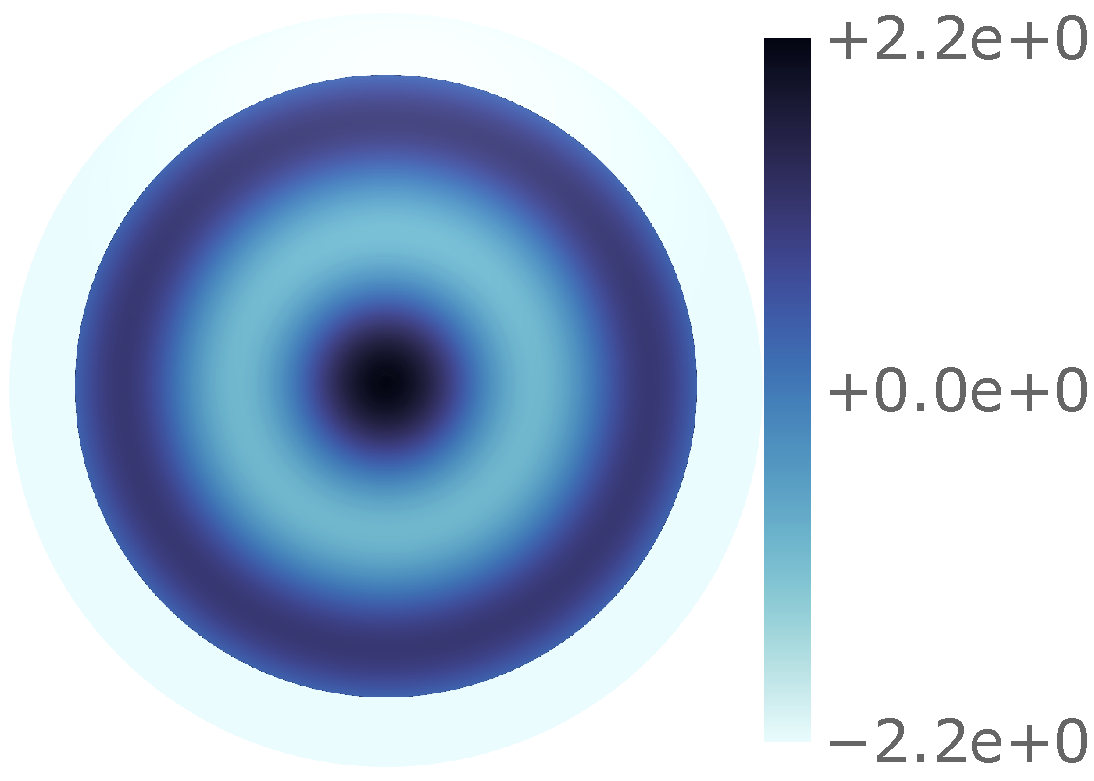
\includegraphics[trim={23 7 3 6},clip,width=.25\textwidth]{slepian_polar40_m0_rank14_lam9-846542e-01_L16_res128_real.pdf}} % chktex 8
	\hfill
	\subfloat[\(\mu_{16}=0.973439\)]
	{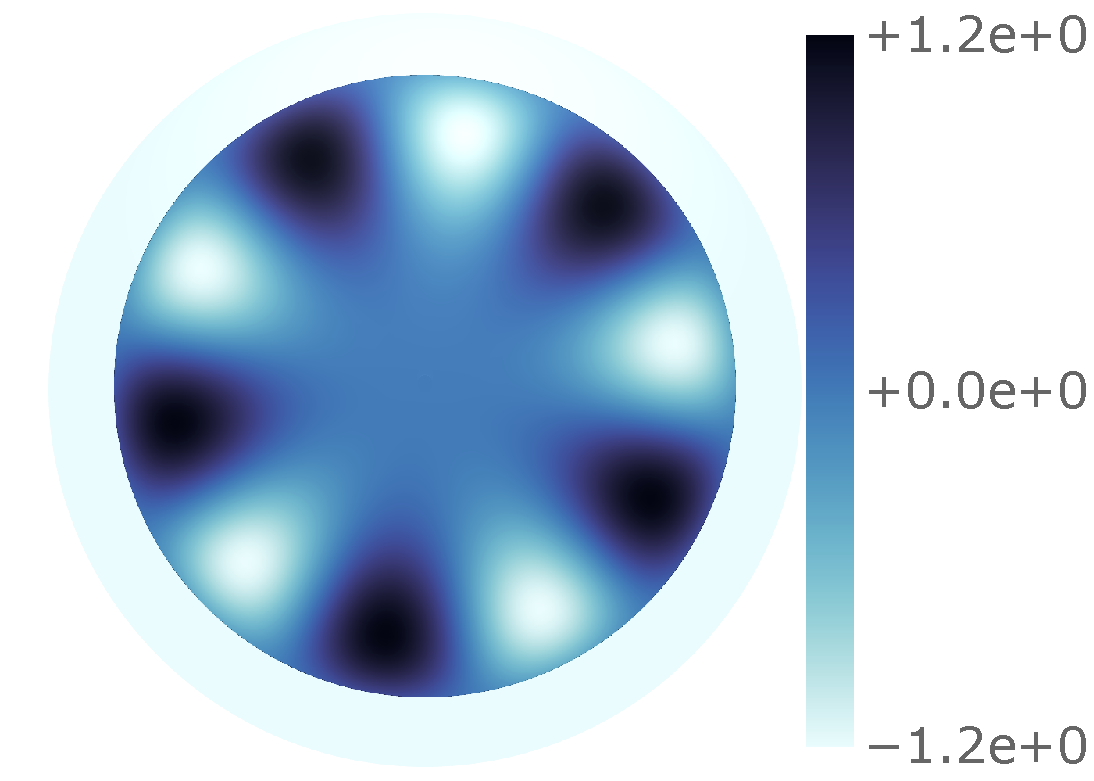
\includegraphics[trim={23 7 3 6},clip,width=.25\textwidth]{slepian_polar40_m5_rank15_lam9-734390e-01_L16_res128_real.pdf}} % chktex 8
	\caption[
		The Slepian functions within a \(\SI{40}{\degree}\) polar cap
	]{
		The first sixteen Slepian functions \(\pixel{\slepian{S}}\) within a polar cap of colatitudinal radius \(\Theta=\SI{40}{\degree}\).
		The bandlimit here is  \(L=16\), which corresponds to a Shannon number of \(N=30\).
		Ordered by decreasing eigenvalue, the plots are shown left-to-right, top-to-bottom --- indicating worse concentration within the region.
		Note the similarity with the spherical harmonics in this straightforward region.
	}\label{fig:chapter2_slepian_polar_cap}
\end{figure}
